\documentclass{beamer}
\usepackage[swedish]{babel}
\usepackage[utf8]{inputenc}
\usepackage[utf8]{inputenc}
\usepackage{amsmath}
\usepackage{amssymb}
\usepackage{amsthm}
\usepackage{graphicx}

\uselanguage{swedish}
\languagepath{swedish}
\deftranslation[to=swedish]{Theorem}{Sats}
\deftranslation[to=swedish]{theorem}{sats}
\deftranslation[to=swedish]{Example}{Exempel}
\deftranslation[to=swedish]{example}{exempel}




\usetheme{Warsaw}

\title[Algoritmer och komplexitet inom algebraisk geometri]{
	Algoritmer och komplexitet inom \\
	kommutativ algebra \& algebraisk geometri \\[20pt]
	\large Omparametrisering av kurvor, semigrupper, \\
	implicit notation \& multiplicitetsföljder}

\author[Peter Waher]{Peter Waher \\[10pt]
	\texttt{peterwaher@hotmail.com}\\
	\texttt{https://github.com/PeterWaher/Algebraiska\_kurvor}}

\begin{document}

\begin{frame}
	\titlepage
\end{frame}

\begin{frame}
	\frametitle{Outline}
	\tableofcontents[pausesections]
\end{frame}

\section{Plana algebraiska kurvor}
\subsection{Introduktion}

\begin{frame}
\frametitle{Vad är en plan kurva?}
\begin{Definition}
	En \textbf{plan kurva} $C$ är en delmängd i $\mathbb{C}^2$ sådan att det finns två kontinuerliga funktioner $f : \mathbb{C} \rightarrow \mathbb{C}$ och 
	$g : \mathbb{C} \rightarrow \mathbb{C}$ sådana att $C = \left\{\left(f(t), g(t)\right) : t \in \mathbb{C}\right\}$. $(f, g)$ är en \textbf{parametrisering} av $C$. Om $C$ kan parametriseras av två analytiska funktioner $f$ och $g$ kallas $C$ \textbf{analytisk}. Om den kan parametriseras av två polynom kallas $C$ för \textbf{algebraisk}. Om den kan parametriseras av två formella potensserier kallas $C$ \textbf{algebroid}.
\end{Definition}
\end{frame}

\begin{frame}
	\frametitle{Kurvor i det Euklidiska planet}
	Traditionellt har man ofta studerat plana kurvor i det \emph{Euklidiska planet}. I detta fall är kurvan parametriserad av reellvärda funktioner $f : \mathbb{R} \rightarrow \mathbb{R}$ och 
	$g : \mathbb{R} \rightarrow \mathbb{R}$.
	
  	\begin{example}
		\begin{columns}[onlytextwidth]
			\begin{column}{0.5\textwidth}
				\[C(t)=(t^2,t^3+t^7)\]\\[20pt]
				\scriptsize Not: För att förenkla notationen kan vi identifiera kurvan $C$ med en viss parametrisering $(f, g)$, även om parametriseringen inte är unik. Detta görs enklast genom att identifiera kurvan med funktionen $C : \mathbb{C} \rightarrow \mathbb{C}^2$, $C(t) = \left(f(t), g(t)\right)$. Notera dock att kurvan som sådan och en av dess parametriseringar är två olika objekt.
			\end{column}
			\begin{column}{0.5\textwidth}
				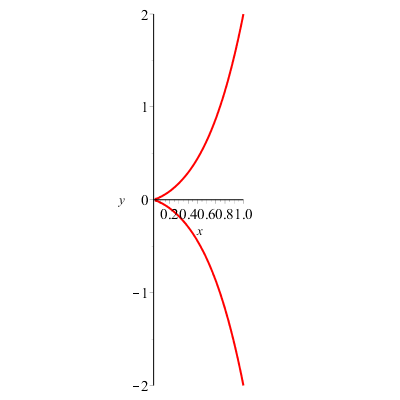
\includegraphics[scale=0.35]{Export/blowupex1_1.png}
			\end{column}
		\end{columns}
  	\end{example}
\end{frame}


\begin{frame}
	\frametitle{Förenklingar}
	Förenklingar vi kan göra om vi studerar en plan kurva lokalt:
	
	\begin{enumerate}
		\item<1-> Tillräckligt att studera \emph{algebraiska} kurvor:
		\begin{enumerate}
			\item<2-> Analytiska funktioner kan skrivas som formella potensserier kring den punkt vi studerar.
			\item<3-> Formella potensserier kan approximeras av polynom med önskad noggrannhet.
		\end{enumerate}
		\item<4-> Kurvan går genom \emph{origo}: $C(0) = \mathbf{0}$
	\end{enumerate}
\end{frame}

\begin{frame}
	\frametitle{Reguljära och singulära kurvor}
\begin{Definition}
	Om en kurva $C$ har en parametrisering $(f, g)$ sådan att $f'(0) \neq 0$ eller $g'(0) \neq 0$ kallas kurvan \textbf{reguljär}. Annars kallas kurvan \textbf{singulär}.
\end{Definition}

\vspace{20pt}
\scriptsize Not: Bara för att $f'(0) = 0$ och $g'(0) = 0$ i en parametrisering $(f, g)$ av en kurva $C$, betyder inte det att kurvan är singulär. Det kan ju finnas en parametrisering av samma kurva där någon av derivatorna är nollskilda. Exempelvis är $(t^3, t^3)$ och $(t, t)$ två olika parametriseringar av samma kurva. I det första exemplet är derivatorna $0$ i origo medan de i det andra exemplet båda är nollskilda.
\end{frame}

\begin{frame}
	\frametitle{Ordning och grad}
\begin{Definition}
	\textbf{Ordningen} av ett polynom eller en potensserie $f(t) =
	\sum a_i t^i \neq 0$ är det minsta heltalet $k$ sådant att koefficienten $a_k$ är nollskild, och skrivs $\mathbf{o}(f)$. \textbf{Graden} for motsvarande polynom är det största heltalet $k$ sådant att koefficienten $a_k$ inte är noll, och skrivs $\deg(f)$.
\end{Definition}
\end{frame}

\subsection{Omparametrisering}

\begin{frame}
	\frametitle{Varför omparametrisera?}
	\begin{enumerate}
		\item För utritande av kurvor spelar parametriseringen inte så stor roll.
		
		\item Vill man beräkna $y(x) = g(f^{-1}(x))$ eller $x(y) = f(g^{-1}(y))$, står man genast inför en mängd problem.
	\end{enumerate}
\end{frame}

\begin{frame}
	\frametitle{Omparametrisering av kurvor}
\begin{Theorem}
	\label{ReparametrizeTheorem}
	Om $C = C(t) = \left(f(t), g(t)\right)$ är en komplex analytisk, algebroid eller algebraisk kurva, samt att $f(0) = g(0) = 0$, kan kurvan $C$ omparametriseras på formen $C^*(t) = \left(\pm t^n, g^*(t)\right)$ eller på formen $C^*(t) = \left(f^*(t), \pm t^n \right)$ i ett område kring $t = 0$, där $f(t)$ och $g(t)$ är formella potensserier. Dessutom gäller att $\mathbf{o}\left(f^*\right) \geq n$ eller att $\mathbf{o}\left(g^*\right) \geq n$. Om $f(t)$ och $g(t)$ är reellvärda, kan också omparametriseringen göras reellvärd.
\end{Theorem}

\vspace{20pt}
\scriptsize Not: Från \emph{Weierstrass Preparation Theorem} får man att en sådan omparametrisering existerar. Dock presenteras inte en metod över hur en sådan omparametrisering kan tas fram.
\end{frame}

\begin{frame}
	\frametitle{Bevisdisposition}
	Beviset av satsen går igenom följande steg:
	
	\begin{enumerate}
		\item<1-> Vi skapar en omparametrisering via komposition med $\phi(t)$:
		\[C^*(t) = (f^*(t), g^*(t)) = (f(\phi(t)), g(\phi(t)))\]
		
		\item<2-> Vi väljer $\phi(t)$ sådan att:
		\begin{enumerate}
			\item<3-> Analytisk kring $t = 0$.
			
			\item<4-> $\phi(0)=0$
			
			\item<5-> $\mathbf{o}(\phi)=1 \Longrightarrow \mathbf{o}(f(\phi))=\mathbf{o}(f) \wedge \mathbf{o}(g(\phi))=\mathbf{o}(g)$
			
			\item<6-> $\phi(t), f(t), g(t)$ reellvärda $\Longrightarrow$ $C^*(t)$ reellvärd.
			
		\end{enumerate}
		
		\item<7-> Med början i $a_1$, löses koefficienterna $a_i$ ut ur $\phi(t)=\sum_{k=1}^{\infty}a_k t^k$ för att uppfylla ovanstående.
		
		\item<8-> Finns precis en lösning i det generella fallet som uppfyller ovanstående samt satsens krav.
		
	\end{enumerate}
\end{frame}

\begin{frame}
	\frametitle{\texttt{Reparametrize()}}
\end{frame}

\begin{frame}
	\frametitle{}
\end{frame}

\begin{frame}
	\frametitle{}
\end{frame}

\begin{frame}
	\frametitle{}
\end{frame}


\section{Semigrupper}
\subsection{Definitioner}
\subsection{Beräkning av konduktören}
\subsection{Polynomringen $\mathbb{C}[t]$ och dess delringar}
\subsection{Semigrupper för $\mathbb{C}[p_1,\ldots,p_n]$}

\section{Implicit notation}

\section{Multiplicitetsföljder}
\subsection{Uppblåsningar}
\subsection{Multiplicitetsföljder \& funktionsfamiljer}
\subsection{Komplexitet}

\end{document}